\part{On-Shell Approach to \\
	Scattering $\mathcal{A}$mplitudes}
% 计数器清零,每个part都要引用,除了part1
\setcounter{theorem}{0}
\setcounter{definition}{0}
\setcounter{lemma}{0}
\setcounter{sidenote}{1}

散射振幅的学习笔记,重点在double copy,前面一些基础内容主要参考\cite{Elvang:2015rqa}和张扬老师的线上note\sn{\url{http://staff.ustc.edu.cn/~yzhphy/PH16212.html}},后面double copy主要参考\cite{Carrasco:2015iwa,Bern:2019prr,Bern:2022wqg}。

这部分一个重要的Motivation就是微扰论计算QCD胶子散射过程,即便是纯胶子(纯YM)的树级振幅\sn{不需要考虑鬼场和其他粒子相互作用顶点,只需要关注胶子三顶角和四顶角,没有圈图还不需要做重整化},需要计算的费曼图的数目随外线数目的增长远超阶乘!如果考虑圈图以及其他粒子相互作用,就更为复杂。这个时候再执着于用传统的微扰论,也就是费曼图方法去计算散射振幅已经没有出路了。而传统的费曼图方法是用理论的拉氏量路径积分围绕展开导出的,规范场的拉氏量最大的特点就是存在规范冗余。实际上,虽然要计算的图非常多,但是在计算的最后将在壳条件$p^2=0$以及横向极化条件$p\cdot\epsilon^{\pm}=0$代入之后,相当多的项直接为0。所以,现代散射振幅的计算发展出一套在壳方法,始终带着这两个条件进行计算,脱离拉氏量本身,这会让计算变得容易很多。本note主要关注于树图散射振幅的现代在壳纲领。
\section{Color Decomposition of Gluon Amplitudes}
Yang-Mill理论的拉氏量为:
\begin{equation}
	\begin{aligned}
		\mathcal{L}=-\frac14\operatorname{Tr}F_{\mu\nu}F^{\mu\nu}\\
		\begin{aligned}F_{\mu\nu}=\partial_{\mu}A_{\nu}-\partial_{\nu}A_{\mu}-\frac{ig}{\sqrt{2}}[A_{\mu},A_{\nu}]\end{aligned}
	\end{aligned}
\end{equation}
这里出现的$\sqrt{2}$是因为我们选取了$\mathrm{Tr~}T^aT^b=\delta^{ab}$的归一化,常见的也有$\mathrm{Tr~}T^aT^b=\frac{1}{2}\delta^{ab}$的选择。传统微扰计算振幅的第一步就是加入规范固定项和鬼场,由于考虑的只是树级振幅,所以后者不需要了。Gervais–Neveu规范在树图层面上非常方便:
\begin{equation}
	\mathcal{L}_{\mathrm{gf}}=-\frac12\text{ Tr}({H_{\mu}}^{\mu})^2,\quad H_{\mu\nu}=\partial_{\mu}A_{\nu}-\frac{ig}{\sqrt2}A_{\mu}A_{\nu}
\end{equation}
最终拉氏量为:
\begin{equation}
	\mathcal{L}=\mathrm{Tr}\left(-\frac12\partial_{\mu}A_{\nu}\partial^{\mu}A^{\nu}-i\sqrt{2}g\partial^{\mu}A^{\nu}A_{\nu}A_{\mu}+\frac{g^2}4A^{\mu}A^{\nu}A_{\nu}A_{\mu}\right)
\end{equation}

QCD过程复杂的是顶角函数都会含有色因子,从费曼规则上看他们是和动力学参数动量这些耦合在一起的,这导致最终计算上除了运动学,还要关注色因子求和,非常麻烦。但是在树图阶,色和动力学是解耦的,问题的关键在于下面的完备性关系:\sn{在基本表示下成立,不过QCD就是取的基本表示}
\begin{equation}
	(T^a)_i^j(T^a)_k^l={\delta_i}^l{\delta_k}^j-\frac1N{\delta_i}^j{\delta_k}^l
\end{equation}
\begin{remark}
	这个完备性关系可以用下面形象的图表达:
	\begin{figure}[H]
		\centering
		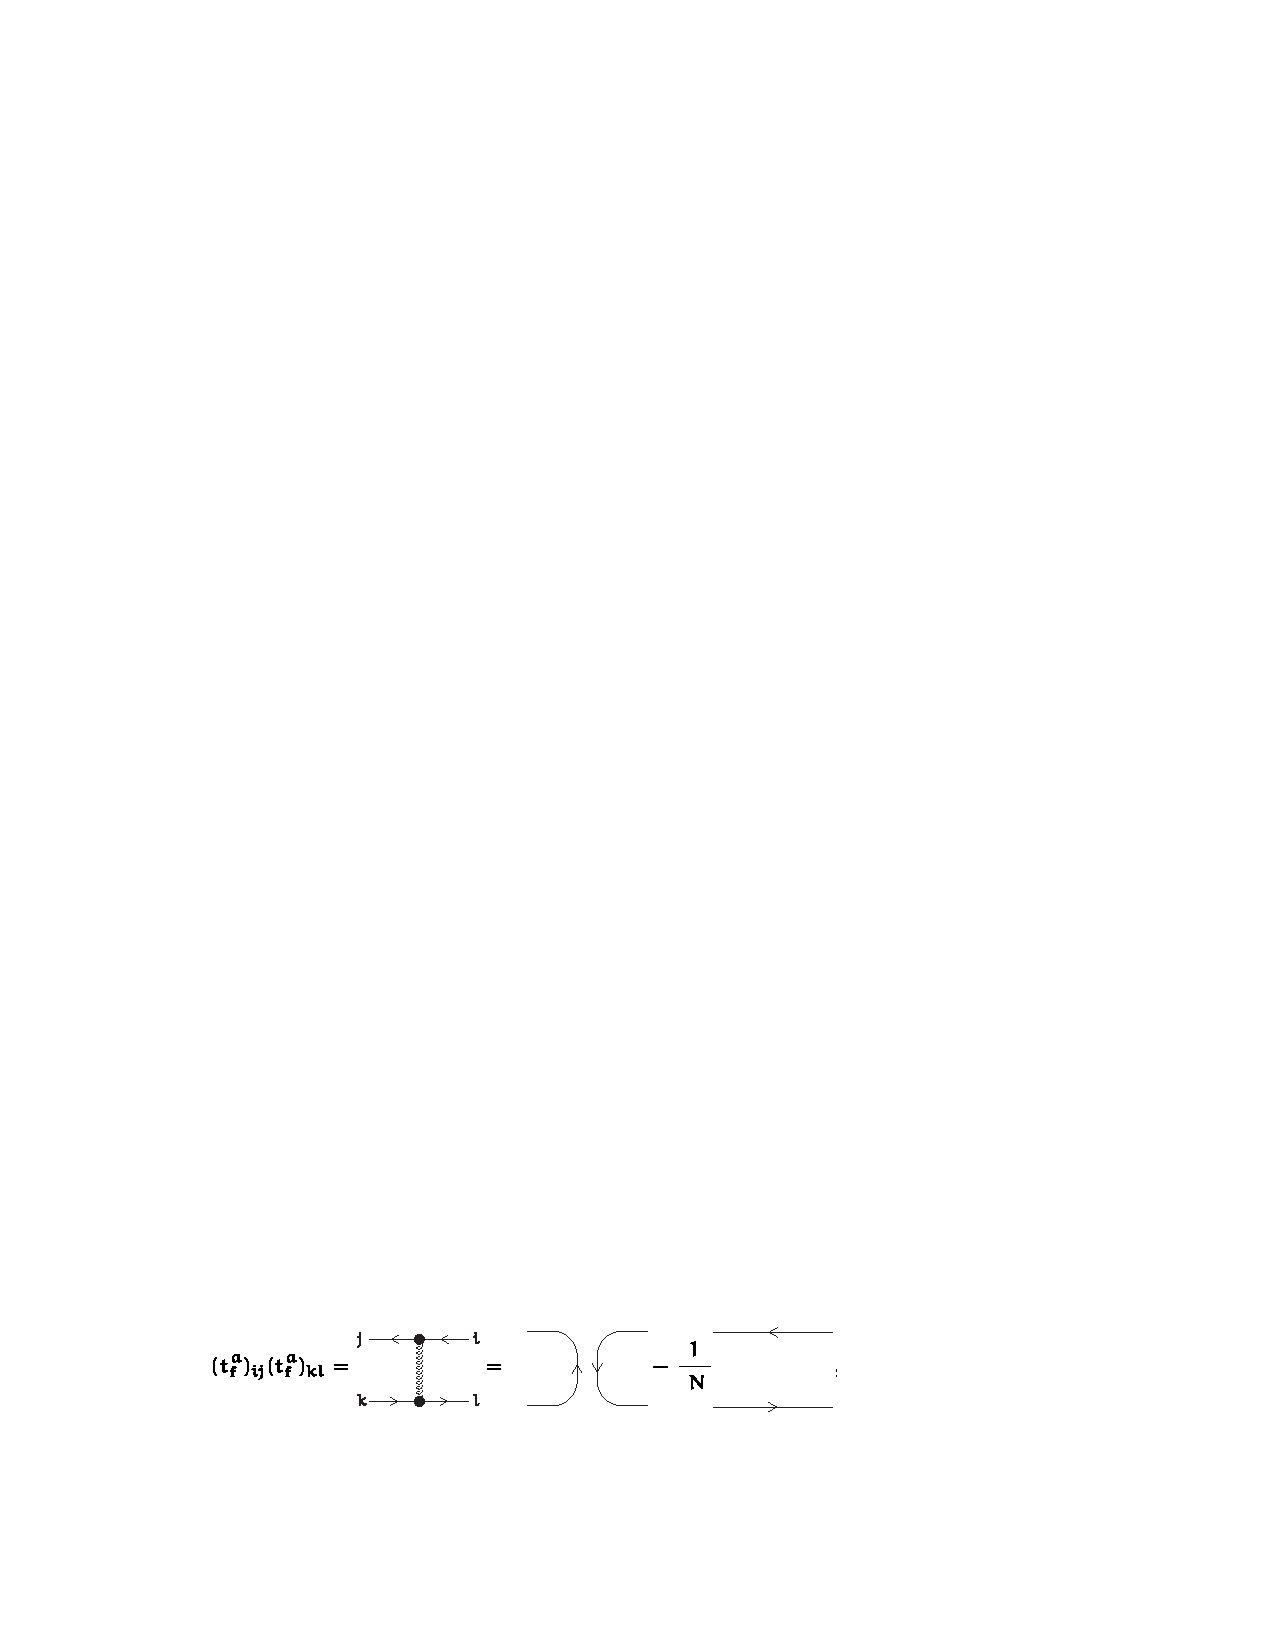
\includegraphics{figs/fig18.pdf}
	\end{figure}
	粗黑点表示一个生成元矩阵,胶子线表示色因子求和,外线表示矩阵下标,相连表示求和。这种类似Penrose张量图示的方法非常直观,甚至书籍\cite{cvitanovic_group_2008}就全篇用这个记号讲群论。比如下面的化简就可以用图的方法证明:
	\begin{figure}[H]
		\centering
		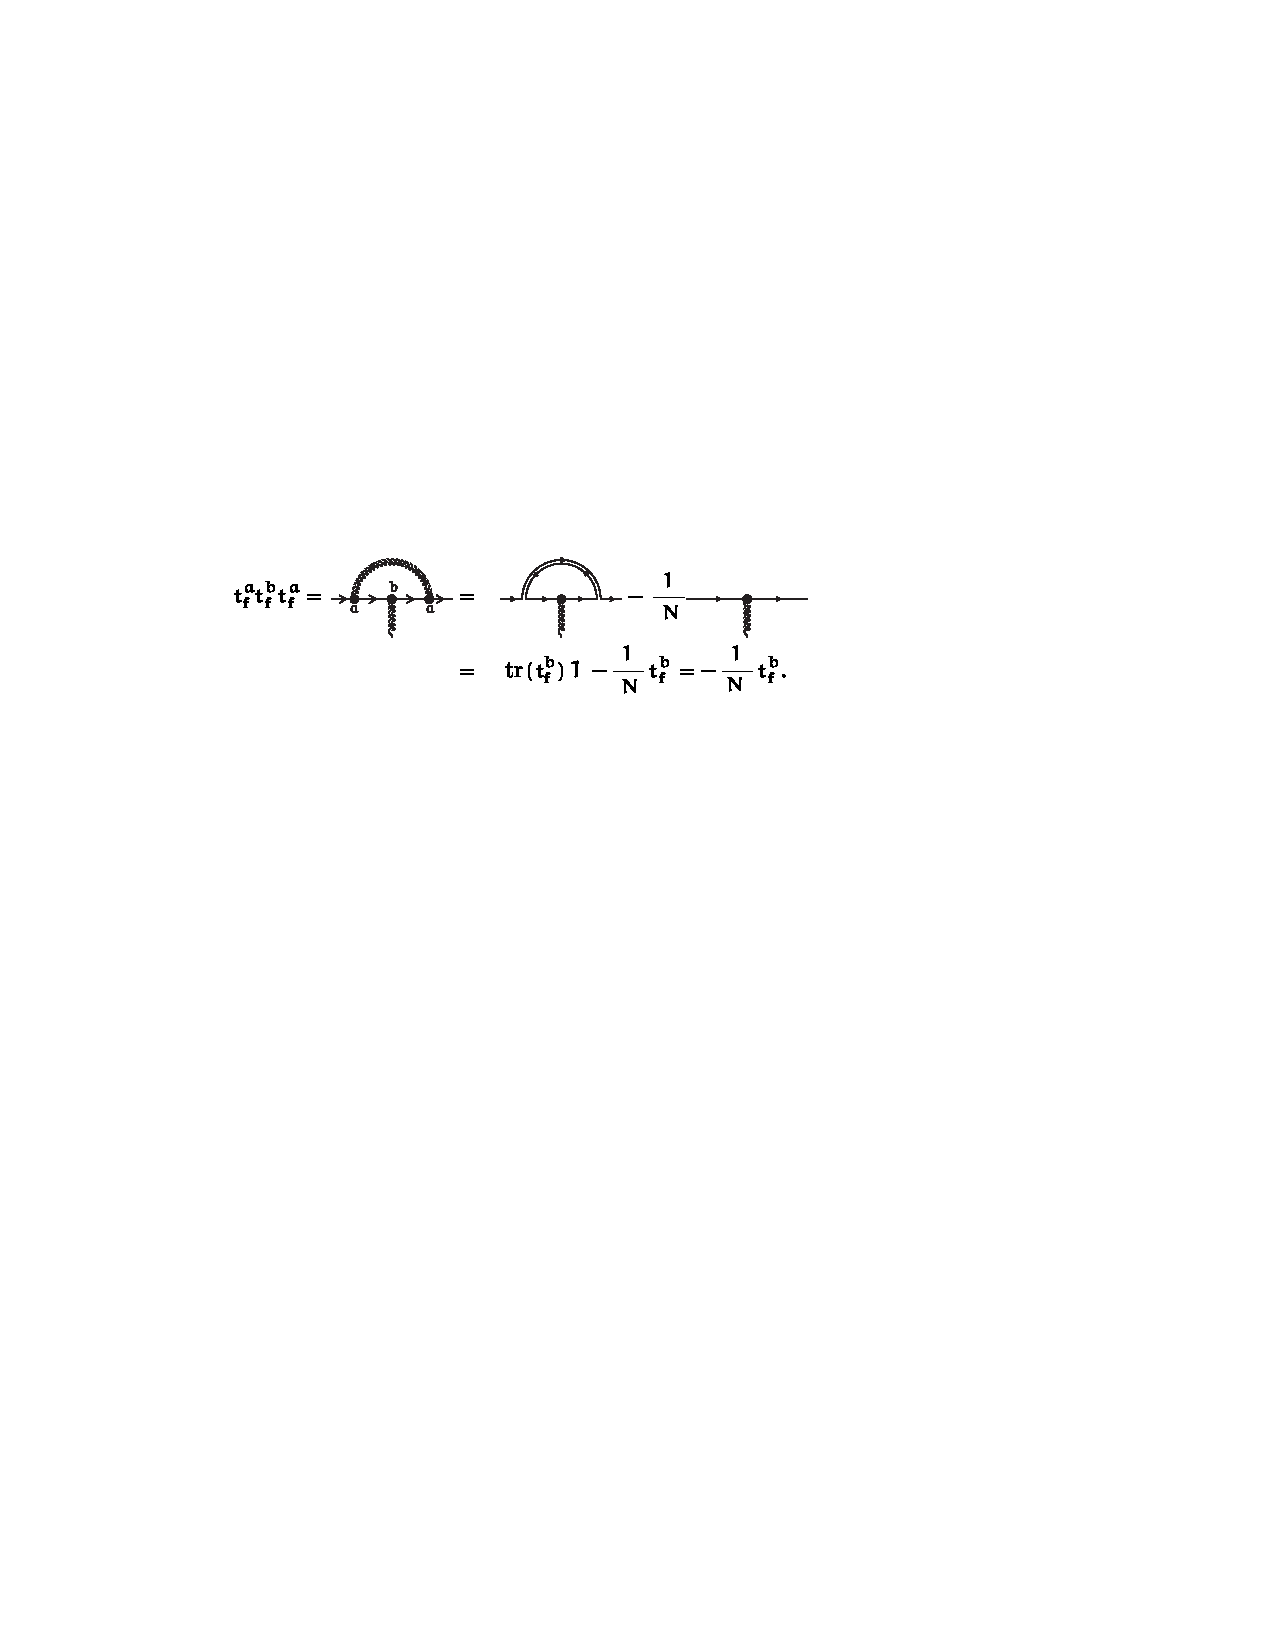
\includegraphics{figs/fig19.pdf}
	\end{figure}
	\cite{Gelis:2019yfm}用这种图证明了四点情况的色因子分解。
\end{remark}
由此可以把任意树图阶振幅写成下面的形式:
\begin{equation}
	\mathcal{A}_n^{\mathrm{full,tree}}=g^{n-2}\sum_{\sigma\in\mathfrak{S}_n/\mathbb{Z}_n}\operatorname{tr}\Big(T^{a_{\sigma(1)}}\cdots T^{a_{\sigma(n)}}\Big)A_n(\sigma(1)\cdots\sigma(n))
\end{equation}
这里$\mathfrak{S}_n/\mathbb{Z}_n$的意思是所有指标的置换商掉轮换。这也等价于第一个指标不动,后面的指标轮换:
\begin{equation}
	\mathcal{A}_n^{\mathrm{full,tree}}=g^{n-2}\sum_{\text{perms }\sigma}A_n{\left[1\sigma(2\ldots n)\right]\mathrm{Tr}\left(T^{a_1}T^{\sigma(a_2}\cdots T^{a_n)}\right)}
\end{equation}
不难发现,色因子完全蕴含在前面一堆生成元的Trace中,我们唯一要去计算的就是$A_n(\sigma(1)\cdots\sigma(n))$,称为\textbf{色序偏振幅},之和胶子的动量以及螺旋度有关。

色序偏振幅有下面的特性:
\begin{itemize}
	\item 轮换性:
	\begin{equation}
		A_n[12\ldots n]=A_n[2\ldots n1]
	\end{equation}
	\item 对称性:
	\begin{equation}
		A_n[12\ldots n]=(-1)^nA_n[n\ldots21].
	\end{equation}
	\item U(1)光子解耦公式:
	\begin{equation}
		A_n[123\ldots n]+A_n[213\ldots n]+A_n[231\ldots n]+\cdots+A_n[23\ldots1n]=0
	\end{equation}
\end{itemize}
最后一个等式的证明非常精妙,它来源于胶子不和光子相互作用,没有U(1)的项,把其中一个$T^a$换成恒等元一定会导致振幅为0。
\subsection{Color-Ordered Feynman Rules}
提出色因子之后需要计算的图大量减少,\textbf{只要那些平面图才会对色序偏振幅有贡献}\sn{\begin{equation*}
		\begin{array}{|l|r|r|}\hline\text{胶子的数目}&\text{图的数目}&\text{轮换序图的数目}\\\hline4&4&3\\\hline5&25&10\\\hline6&220&38\\\hline7&2,485&154\\\hline8&34,300&654\\\hline9&589,405&2.871\\\hline10&10,525,900&12.925\\\hline\end{array}
\end{equation*}}。比如四点振幅,有贡献的是下面三个图:
\begin{equation}
	A_4(1234)=\feynmandiagram [horizontal=a to b,layered layout,inline=(a.base)] [small,edges=gluon] {
		{i1[particle=\(1\)], i2[particle=\(2\)]} -- a -- b -- {f1[particle=\(3\)], f2[particle=\(4\)]},
	};+
	\feynmandiagram [vertical=a to b,layered layout,baseline={(current bounding box.center)}] [small,edges=gluon] {
		{i1[particle=\(4\)], i2[particle=\(1\)]} -- a -- b -- {f2[particle=\(2\)], f1[particle=\(3\)]},
	};+
	\feynmandiagram [horizontal=i1 to f2,layered layout,inline=(a)] [small,edges=gluon] {
		{i1[particle=\(2\)], i2[particle=\(4\)]} -- a  -- {f1[particle=\(1\)], f2[particle=\(3\)]},
	};
\end{equation}
下面的这个图是没有贡献的:\sn{这个图用tikz画起来很费劲,参考:\url{https://tex.stackexchange.com/questions/515275/how-do-you-do-crossed-lines-using-tikz-feynman}}
\begin{center}
	\feynmandiagram[horizontal=i1 to i2,remember picture]{
		f1[particle=\(1\)]--[gluon]b--[gluon,
		opacity=0]f2[particle=\(4\)],
		i1[particle=\(2\)]--[gluon]a--[gluon,opacity=0]i2[particle=\(3\)],
		b--[gluon]a,
	};
	
	\begin{tikzpicture}[overlay,remember picture]
		\begin{feynman}
			\path (b) -- (i2) coordinate[midway] (b1)
			(a) -- (f2) coordinate[midway] (a1);
			\diagram*{
				(b) --[gluon] (b1) -- [gluon] (i2),
				(a) --[gluon] (a1) -- [gluon] (f2)
			};
		\end{feynman}
	\end{tikzpicture}
\end{center}
所以我们干脆画费曼图的时候就直接画那些平面图,我们称为\textbf{轮换序图(cyclic-ordered
graphs)}:
\begin{figure}[H]
	\centering
	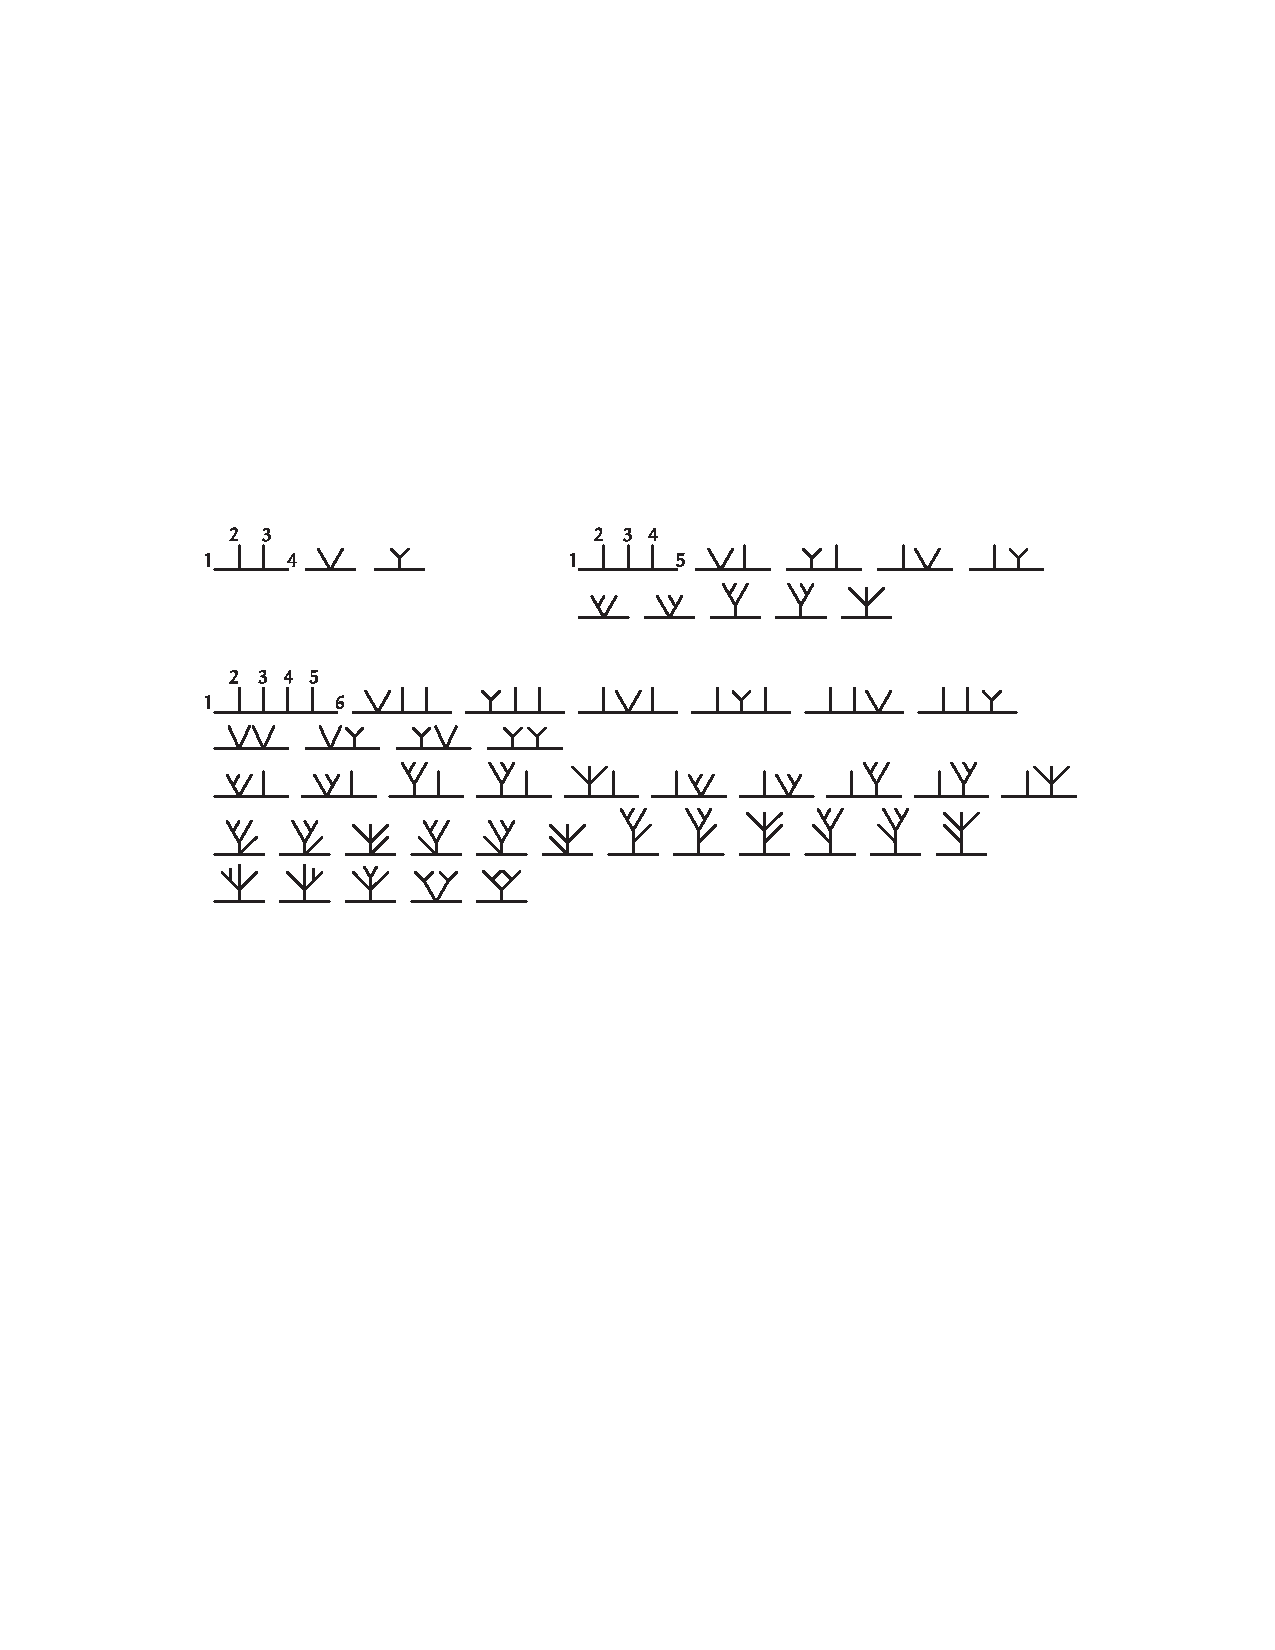
\includegraphics[width=\linewidth]{figs/fig15.pdf}
	\caption{轮换序图}
\end{figure}
计算时使用色序振幅的费曼规则:\sn{$(-+++)$度规,动量参考正方向全部朝外}
\begin{itemize}
	\item 传播子:
	\begin{equation}
		\frac{1}{i}\Delta_{\mu\nu}=\frac{g_{\mu\nu}}{k^2-i\epsilon}+\frac i{p^2-i0^+}\left(1-\frac1\xi\right)\frac{p_{\mu}p_{\nu}}{p^2}
	\end{equation}
	\item 3-pt:
	\begin{equation}
		iV^{\mu_1\mu_2\mu_3}(p_1,p_2,p_3)=-i\sqrt{2}\left(g^{\mu_1\mu_2}p_1^{\mu_3}+g^{\mu_2\mu_3}p_2^{\mu_1}+g^{\mu_3\mu_1}p_3^{\mu_2}\right)
	\end{equation}
	\item 4-pt:
	\begin{equation}
		iV^{\mu_1\mu_2\mu_3\mu_4}(p_1,p_2,p_3,p_4)=ig^{\mu_1\mu_3}g^{\mu_2\mu_4}
	\end{equation}
\end{itemize}
但是我们仍旧有非常多的项需要计算,为了进一步简化,从而从振幅中迅速读出物理信息,我们需要借助旋量螺旋度形式。
\section{spinor helicity formalism}
任何一个四动量都可以将其改写成一个$2\times 2$的矩阵:
\begin{equation}
	p_{a\dot b}\equiv p_{\mu}\left(\sigma^{\mu}\right)_{a\dot b}=\begin{pmatrix}-p^0+p^3&p^1-ip^2\\p^1+ip^2&-p^0-p^3\end{pmatrix}
\end{equation}
利用$\varepsilon^{ab}$升降指标\sn{\[\begin{aligned}
		&\varepsilon^{12}=\varepsilon^{\dot{1}\dot{2}}=\varepsilon_{21}=\varepsilon_{\dot{2}\dot{1}}=+1,\\
		&\varepsilon^{21}=\varepsilon^{\dot{2}\dot{1}}=\varepsilon_{12}=\varepsilon_{\dot{1}\dot{2}}=-1
	\end{aligned}\]}后可定义$p^{\dot{a}b}\equiv p_{\mu}(\bar{\sigma}^{\mu})^{\dot{a}b}$,不难发现$\det p=-p^2=m^2$,所以对于无质量粒子,上面的矩阵是降秩的,可以拆分为两个向量的外积,我们记为:
\begin{equation}
	\boxed{
		p_{a\dot b}=-|p]_a\left<p\right|_{\dot b},\quad p^{\dot{a}b}=-|p\rangle^{\dot{a}}\left[p\right|^b
	}
\end{equation}
$|\cdot],|\cdot\rangle$这些就是旋量螺旋度形式,不难发现他们隐含$\det p=0$,在壳条件被自动满足。根据$\gamma$矩阵的表达式:
\begin{equation}
	-\slashed{p}=-\begin{pmatrix}0&p_{a\dot{b}}\\p^{\dot{a}b}&0\end{pmatrix}=|p\rangle[p|+|p]\langle p|
\end{equation}
注意,上面的式子最后一个等号要理解为在左右手征的投影下成立,毕竟左边是$4\times 4$的矩阵,到了右边变成了$2\times2$的矩阵。或者说把不加下标的旋量螺旋度形式看成是增广矩阵:
\begin{equation}
	[p|\equiv\left([p|^a,0\right)\quad
	\bra{p}\equiv \left(0,\bra{p}_{\dot a}\right)\quad
	|p]\equiv \begin{pmatrix}|p]_a\\0\end{pmatrix}\quad
	\ket{p}\equiv\begin{pmatrix}0\\|p\rangle^{\dot{a}}\end{pmatrix}\quad
\end{equation}
后面经常两种混用\sn{这种混用不会对后面的恒等式产生任何影响,而且这种四分量的形式相比于两分量的形式能提醒我们单独的$\ket{\cdot}$和$|\cdot]$不能形成内积}。$p_{a\dot b}\to p^{\dot a b}$可以翻译为:
\begin{equation}\label{43.4}
\boxed{
	[p|^a=\epsilon^{ab}|p]_b,\quad|p\rangle^{\dot{a}}=\epsilon^{\dot{a}\dot{b}}\langle p|_{\dot{b}}
}
\end{equation}
\begin{theorem}
	\begin{equation}\label{43.5}
		p^\mu\text{ real}:\quad[p|^a=(|p\rangle^a)^*\quad\text{ and }\quad\langle p|_{\dot{a}}=(|p]_a)^*
	\end{equation}
\end{theorem}
\begin{proof}
	注意这里动量为实数的要求并不是废话,证明BCFW递推的时候就需要要把它shift到复平面上去。此式的证明只需要将旋量螺旋度形式用四动量写出来就好了,比如:
	\[|p\rangle^{\dot{a}}=\sqrt{2E}\begin{pmatrix}\cos\frac\theta2\\\sin\frac\theta2e^{i\phi}\end{pmatrix}\]
	其中:
	\[p^\mu=(E,E\sin\theta\cos\phi,E\sin\theta\sin\phi,E\cos\theta)\]
\end{proof}
定义下面的内积:
\begin{equation}
	\langle pq\rangle=\langle p|_{\dot{a}}|q\rangle^{\dot{a}},\quad[pq]=[p|^{a}|q]_{a}
\end{equation}
利用\ref{43.4}还可以证明这个内积是反对称的:
\begin{equation}
	\langle pq\rangle=-\langle qp\rangle,\quad[pq]=-[qp]
\end{equation}
所以有下面的等式:
\begin{equation}\label{43.9}
	p^{\dot{a}b}|p]_b=0,\quad\left.p_{a\dot{b}}|p\right>^{\dot{b}}=0,\quad\left[p\right|^bp_{b\dot{a}}=0,\quad\left<p\right|_{\dot{b}}p^{\dot{b}a}=0
\end{equation}
根据\ref{43.5}还有等式:
\begin{equation}\label{43.10}
	\left\langle pq\right\rangle =[qp]^*
\end{equation}
在进一步分析之前,强调一下目前为止我们对旋量螺旋度形式的介绍完全是数学上的操作,但他们其实是有物理含义的。旋量螺旋度形式完全可以从物理动机上引入。Dirac方程在无质量极限下形式为:\sn{$\bar\cdot = \gamma^0(\cdot)^\dagger$,$v,\bar u$表示出射反费米子和费米子}
\begin{equation}
	\slashed{p}v_{\pm}(p)=0,\quad\bar u_{\pm}\slashed{p}=0
\end{equation}
在Weyl基底下上面无质量Dirac方程的解左右手完全分开,所以我们可以将解设为:
\begin{equation}\label{43.12}
	\begin{aligned}v_+(p)&=\begin{pmatrix}|p]_a\\0\end{pmatrix},\quad&v_-(p)=\begin{pmatrix}0\\|p\rangle^a\end{pmatrix},\\\overline{u}_-(p)&=\left(0,\langle p|_a\right),\quad&\overline{u}_+(p)=\left(\left[p\right|^a,0\right)\end{aligned}
\end{equation}
无质量极限下交叉对称性保证$u_\pm=v_\mp,\bar u_\pm =\bar v_\mp$,而这正是\ref{43.4}。\ref{43.9}就是Dirac方程。由此可见旋量螺旋度形式是有非常清晰的物理意义的,在设计无质量费米子的散射问题时,我们也可以直接使用\ref{43.12}的替换来在壳地计算散射振幅,由于此时非常简单的交叉对称性,默认计算散射振幅时所有的外线都是出射粒子。

下面是一些常用的恒等式:
\begin{equation}
	\langle p q\rangle[p q]=2p\cdot q=(p+q)^2
\end{equation}
下式中的旋量螺旋度形式作四分量形式理解,或者看作两分量,但是$\gamma$理解成把左右手征的sigma矩阵抽出来\sn{具体投影到哪一个根据带点旋量指标之间缩并,不带点指标之间缩并}。
\begin{equation}
	\begin{aligned}
		[k|\gamma^\mu\ket{p}&=\bra{p}\gamma^\mu|k],\\ [k|\gamma^\mu\ket{p}^*&=[p|\gamma^\mu\ket{k}\quad\text{($p\in\mathbb{R}^4$)}\\
		\langle p|\gamma^\mu|k\rangle=&0=[p|\gamma^\mu|k]
	\end{aligned}
\end{equation}
Fierz恒等式:
\begin{equation}
	\begin{aligned}-\frac12\langle p|\gamma_\mu|q]\gamma^\mu&=|q]\langle p|+|p\rangle[q|\\[2ex]-\frac12[p|\gamma_\mu|q\rangle\gamma^\mu&=|q\rangle[p|+|p]\langle q|\end{aligned}
\end{equation}
Sandwich一下可以得到:
\begin{equation}
	\langle1|\gamma^\mu|2]\langle3|\gamma_\mu|4]=2\langle13\rangle[24]
\end{equation}
我们经常会使用$i$作为$p_i$的简写。
\begin{equation}
	\sum_{i=1}^n|i\rangle[i|=0,\quad\text{ i.e. }\quad\sum_{i=1}^n\langle qi\rangle[ik]=0
\end{equation}
这个式子实际上是动量守恒,$q,k$的选取是任意的。由于任意的二分量旋量空间最大独立的旋量个数只能是2,所以有Schouten恒等式:
\begin{equation}
	|i\rangle\langle jk\rangle+|j\rangle\langle ki\rangle+|k\rangle\langle ij\rangle=0
\end{equation}
更常用的形式是将上式左乘一个任意的$\bra{r}$:
\begin{equation}
	\langle ri\rangle\langle jk\rangle+\langle rj\rangle\langle ki\rangle+\langle rk\rangle\langle ij\rangle=0
\end{equation}
利用
\begin{equation}
	\mathrm{Tr}(\sigma^{\mu}\bar{\sigma}^{\nu}\sigma^{\tau}\bar{\sigma}^{\rho})=2(\eta^{\mu\nu}\eta^{\tau\rho}+\eta^{\mu\rho}\eta^{\nu\rho}-\eta^{\mu\tau}\eta^{\nu\rho}+i\epsilon^{\mu\nu\tau\rho})
\end{equation}
可以证明下面的等式:
\begin{equation}
	\langle ij\rangle[jk]\langle kl\rangle[li]=2(p_i\cdot p_l)(p_j\cdot p_k)+2(p_i\cdot p_j)(p_k\cdot p_l)-2(p_i\cdot p_k)(p_j\cdot p_l)-2i\epsilon(i,j,k,l)
\end{equation}
\begin{definition}[Gram matrix]
	任意的四个矢量可以定义出一个Gram矩阵:
	\begin{equation}
		G(e_1,e_2,e_3,e_4)_{ij}\equiv e_i\cdot e_j
	\end{equation}
	由此衍生出一个Lorentz不变量:
	\begin{equation}
		g(e_1,e_2,e_3,e_4)\equiv\det G(e_1,e_2,e_3,e_4)=-\epsilon(i,j,k,l)^2
	\end{equation}
\end{definition}
其中$\epsilon(i,j,k,l)=\epsilon^{\mu_{1}\mu_{2}\mu_{3}\mu_{4}}p_{i\mu_{1}}p_{j\mu_{2}}p_{k\mu_{3}}p_{l\mu_{4}}$。
前面我们只说明了这个符号是在壳的,我们还需要说明横向极化条件也被满足,实际上极化矢量有下面的形式:\sn{出射对应$\epsilon$,入射对应$\epsilon^*$,后面考虑散射全部都是出射}
\begin{equation}
		\boxed{
			\epsilon_{-}^{\mu}(p;q)=-\frac{\langle p|\gamma^{\mu}|q]}{\sqrt{2}[qp]},\quad\epsilon_{+}^{\mu}(p;q)=-\frac{\langle q|\gamma^{\mu}|p]}{\sqrt{2}\langle qp\rangle}
		}
\end{equation}
这里$q$是参考动量,选取是任意的,不会对振幅的计算有任何影响,其实这就相当于$\epsilon_{\pm}^{\mu}(p)\to\epsilon_{\pm}^{\mu}(p)+Cp^{\mu}$,Ward恒等式保证了振幅不受影响。但是这是在所有图求和之后,所以对于一个散射过程的不同图,$q$的选取必须一致。极化适量的slash有下面的形式:
\begin{equation}
	\slashed{\epsilon}_-(p;q)=\frac{\sqrt{2}}{[qp]}\Big(|p\rangle[q|+|q]\langle p|\Big),\quad\slashed{\epsilon}_+(p;q)=frac{\sqrt{2}}{\langle qp\rangle}\Big(|p]\langle q|+|q\rangle[p|\Big)
\end{equation}
\subsection{Little Group Scale}
虽然我们将$p$分解为了两个二分量旋量的外积,但是这种分解方式仍然是存在冗余的:
\begin{equation}
	\begin{aligned}
		&\bra{p}\mapsto z\bra{p},|p]\mapsto z^{-1}|p]\\
		&\ket{p}\mapsto z\ket{p},[p|]\mapsto z^{-1}[p|
	\end{aligned}
\end{equation}
这实际上对应Lorentz群的$ISO(2)$小群变换,对于$p\in\mathbb{R}$,由于\ref{43.4},$|z|=1,z\in\mathbb{C}$。这个对称性对振幅产生的唯一影响就是一个尺度变换。这个尺度变换完全来自于外腿的$u,v,\epsilon$的贡献,螺旋度为负对应的是$\ket{\cdot}$,所以带来$z^{+1}$,螺旋度为正对应$|\cdot]$,所以带来$z^{-1}$。同理,可证明光子的极化矢量会有$z^{\pm2}$的尺度变换。所以振幅在小群变换下的行为为:
\begin{equation}
		\boxed{
			A_n\left(\{|1\rangle,|1],h_1\},\ldots,\{z_i|i\rangle,z_i^{-1}|i],h_i\},\ldots\right)=z_i^{-2h_i}A_n\left(\ldots\{|i\rangle,|i],h_i\}\ldots\right)
		}
\end{equation}
注意这里我们给$z$加上了下标,因为可以对不同的动量做不同的小群变换。

现在来分析最简单的三点振幅,动量守恒得到:
\begin{equation}
	\ket{1}[1|+\ket{2}[2|+\ket{3}[3|=0\Rightarrow\begin{cases}
		\left\langle 12\right\rangle [2|=-\left\langle 13\right\rangle [3|\\
		\left\langle 21\right\rangle [1|=-\left\langle 23\right\rangle [3|
	\end{cases}
\end{equation}
上面的方程有两组解,一组是:
\begin{equation}
	|1]\propto|2]\propto|3]\iff [12]=[23]=[31]=0\quad\text{holomorphic}
\end{equation}
另一组是:
\begin{equation}
	|1\rangle\propto|2\rangle\propto|3\rangle\iff \left\langle 12\right\rangle=\left\langle 23\right\rangle=\left\langle 31\right\rangle \quad\text{anti-holomorphic}
\end{equation}
由于所有的旋量指标要缩并,所以最后三点振幅的形式一定要么是全纯的,要么是反全纯的,而且,因为实动量会导致\ref{43.10},所以实动量同时满足全纯和反全纯,也就是说任意三点无质量振幅在$p\to\mathbb{R}$时都是0。除非振幅是$\phi^3$理论一样与动力学无关的常数\sn{你还可以考虑$(-,+,-,+)$时空,这时虽然动量依旧是实数,但是$\bra{\cdot}$和$|\cdot]$无关了,所以这个时候三点振幅是non-trivial的}。但是研究三点振幅还是有必要的,因为很多n点振幅都会包含三点振幅,我们可以在计算时先将三点部分动量off-shell到复平面,最后取实轴极限。

考虑反全纯部分,我们有下面的ansatz:
\begin{equation}
	A_3{\left(1^{h_1}2^{h_2}3^{h_3}\right)}=c\mathrm{~}\langle12\rangle^{x_{12}}\langle13\rangle^{x_{13}}\langle23\rangle^{x_{23}}
\end{equation}
小群变换要求:
\begin{equation}
	-2h_1=x_{12}+x_{13}\mathrm{~,~}\quad-2h_2=x_{12}+x_{23}\mathrm{~,~}\quad-2h_3=x_{13}+x_{23}
\end{equation}
最终我们完全确定了三点振幅:
\begin{equation}\label{43.33}
	\boxed{
		A_3\big(1^{h_1}2^{h_2}3^{h_3}\big)=c\left<12\right>^{h_3-h_1-h_2}\langle13\rangle^{h_2-h_1-h_3}\langle23\rangle^{h_1-h_2-h_3}
	}
\end{equation}
反全纯部分类似。还有一个问题是如何确定振幅是全纯的还是反全纯的,这可以通过分析质量量纲得到,如果我们从拉氏量清楚振幅的质量量纲,则根据bracket的量纲为1就可以分析出来了。
\begin{theorem}
   D维时空中的n点振幅的质量量纲为$4-D$
\end{theorem}
\begin{proof}
	利用交叉对称性,n点振幅可以看作是$2\to n-2$的散射过程,根据费米黄金规则,散射截面表达式为:
	\begin{equation}
		d\sigma=\frac1{4|\mathbf{k}_1|_\text{CM}{ \sqrt { s }}}|\mathcal{A}|^2d\mathrm{LIPS}_{n-2}(k_1{+}k_2)
	\end{equation}
	其中:
	\begin{equation}
		\begin{aligned}d\text{LIPS}_{n'}(k)&\equiv(2\pi)^4\delta^4(k{-}\sum_{j=1}^{n'}k_i')\prod_{j=1}^{n'}\widetilde{dk'}_j\end{aligned}
	\end{equation}
	量纲分析得到:
	\begin{equation}
		-2=[d\sigma]=-2+2[\mathcal{A}]+2(n-2)-4
	\end{equation}
\end{proof}
另外你还可以从$p\to\mathbb{R}$时振幅趋近0去想,因为\ref{43.33}关于$\left\langle\cdot\right\rangle$是$-h$幂次的,$h$是总的螺旋度,而$p\in\mathbb{R}$时,会让所有的括号都变成0,所以只有在$h\leq 0$时才不会发散。所以$h\leq 0$的时候反全纯,否则全纯。

上面的这些分析最大的特点是普适性,我们没有引入任何的费曼规则,完全是从自洽性进行分析,这种bootstrap的想法甚至能帮助我们重塑理论的拉氏量\sn{比如在线讲义\url{https://www.ph.nat.tum.de/fileadmin/w00bya/t70/Seminar2021/Amplitudes_Sanfilippo.pdf},三点振幅形式加上理论的定域性要求(没有高阶导数项),就可以重塑拉氏量的三点相互作用项。}。。现在我们来考虑YM理论,量纲分析能帮助我们进一步确定振幅。
\begin{theorem}
	\begin{equation}
		A^\text{tree}_n(1^+2^+\ldots n^+)=0\quad\mathrm{and}\quad A^\text{tree}_n(1^-2^+\ldots n^+)=0
	\end{equation}
	\begin{equation}
		A^\text{tree}_n(1^-2^-\ldots n^-)=0\quad\mathrm{and}\quad A^\text{tree}_n(1^+2^-\ldots n^-)=0
	\end{equation}
\end{theorem}
\begin{proof}
	从振幅是洛伦兹标量出发,不难发现振幅都有下面的形式:
	\begin{equation}
		A_n\sim\sum_\text{diagrams}{ \frac { \sum \left ( \prod ( \epsilon _ i \cdot \epsilon _ j ) \right ) \left ( \prod ( \epsilon _ i \cdot k _ j ) \right ) \left ( \prod ( k _ i \cdot k _ j ) \right ) }{ \prod P _ I ^ 2}}
	\end{equation}
	分母表示平方传播子。传播子质量量纲$[\Delta]=-2$,顶角函数$[V_3]=1,[V_4]=0$,对于全部都是三顶角的图:
	\begin{equation}\label{43.39}
		\left[A_n\right]\sim\frac{(\mathrm{mass})^{n-2}}{(\mathrm{mass}^2)^{n-3}}\sim(\mathrm{mass})^{4-n}
	\end{equation}
	不难发现这种图分子量纲最大,其他图量纲都小于$n-2$。接下来注意到:
	\begin{equation}
		\epsilon_{i+}\cdot\epsilon_{j+}\propto\langle q_iq_j\rangle,\quad\epsilon_{i-}\cdot\epsilon_{j-}\propto[q_iq_j],\quad\epsilon_{i-}\cdot\epsilon_{j+}\propto\langle iq_j\rangle[jq_i]
	\end{equation}
	$q_i$是粒子参考动量,在所有图求和之后振幅与其无关,所以我们可以把所有的$q_i$取成相同的$q$,这样对于振幅$A_n(1^+2^+\cdots n^+)$,唯一有贡献的只能是$\epsilon\cdot k$,而这样的项要有$n$个,这直接导致分子的质量量纲至少为$n>n-2$,所以这样的振幅是被禁闭的。继续考虑$A_n(1^-2^+\cdots n^+)$,取$q_2=q_3=\cdots=q_n=p_1$,这导致$\epsilon_{i+}\cdot\epsilon_{j_+}=0=\epsilon_{1-}\cdot\epsilon_{j+}$。这再次导致需要$n$个$\epsilon\cdot k$,导致禁闭。
	
	\setlength{\parindent}{2em}到这里就证明完了,但是这只是意味着树图振幅求和为0,实际上圈图修正后不为0,证明失效的原因在于\ref{43.39}在loop-level上不成立,tree-level上成立是因为加一个外线,只会带来一个顶角和一个传播子,但是loop-level这一点是错的。
\end{proof}
我们还可以利用三点振幅形式来说明光子没有三点自相互作用项。比如全纯部分振幅形式为:
\begin{equation}
	\mathcal{M}(1^+2^+3^+)=c_1[12][23][31],\quad\mathcal{M}(1^+2^+3^-)=c_2\frac{[12]^3}{[23][31]}
\end{equation}
注意这是振幅,而不是色序偏振幅。由于粒子是玻色子,交换任意两个粒子动量应该是对称的(产生湮灭之间满足对易关系),但是上面括号部分是反对称的,所以要么$c=0$.要么理论中不只有一种玻色子,也就是说这些玻色子带色荷,交换的时候把颜色也交换了,$c$带有颜色指标,而且是全反对称的:
\begin{equation}
	\mathcal{M}(1_a^+2_b^+3_c^+)=c_1^{abc}[12][23][31],\quad\mathcal{M}(1_a^+2_b^+3_c^-)=c_2^{abc}\frac{[12]^3}{[23][31]}
\end{equation}
这正好就说明了光子无自相互作用,圈图修正也为0\sn{
		\begin{equation*}
			\feynmandiagram [small,baseline=(d.base), horizontal=d to b] {
			a[particle=\(\gamma\)] -- [boson] b[blob] -- [boson] c[particle=\(\gamma\)],
			b -- [boson] d [particle=\(\gamma\)],
		};
		= 0
		\end{equation*}
	},胶子三点相互作用正比于全反对称结构张量$f^{abc}$。

虽然我们利用本节的旋量螺旋度形式可以很简洁的表达振幅,但是我们更希望用动力学变量直接表示出来,如:
\begin{definition}[Mandelstam variables]
	对于全部是出射粒子的散射过程,Mandelstam变量定义为:
	\begin{equation}
		s_{ij}=-(p_i+p_j)^2,\quad s_{ijk}=-(p_i+p_j+p_k)^2,\quad\text{etc}.
	\end{equation}
\end{definition}
举个实际计算的例子:
\begin{example}
	\begin{equation}
		\begin{aligned}
		\frac{\langle12\rangle\langle34\rangle}{\langle13\rangle\langle24\rangle}& =\frac{\langle12\rangle\langle34\rangle[31][42]}{s_{13}s_{24}}=\frac{\langle21\rangle[13]\langle34\rangle[42]}{s_{13}s_{24}}  \\
		&=\frac{s_{12}s_{34}/2+s_{24}s_{13}/2-s_{23}s_{14}/2}{s_{13}s_{24}}=\frac{s^2/2-t^2/2+(s+t)^2/2}{(s+t)^2} \\
		&=\frac s{s+t}
	\end{aligned}
	\end{equation}
\end{example}
实际上这个计算是non-trivial的,你需要灵活利用前面的那些恒等式。利用更现代的Momentum Twistor方法,可以把这种化简变成机械式的,具体可见文献\cite{Badger:2013gxa}附录。
\subsection{spinor-helicity formalism on the celestial}
\cite{Pasterski:2017ylz}
\section{Tree Amplitudes}


\section{Collinear Limits} 
虽然散射振幅的形式可以很复杂,但是在一些极限情况下会变得很简单,比如软极限下就直接只是在原先振幅前多个因子。还有一类比较重要的极限是共线极限,本节利用旋量螺旋度形式重述(树阶)软定理以及共线极限下振幅形式。两个极限可以用于检验计算的正确性,也可以根据它们反推出非极限情况下的振幅形式(自举法)。下面的讨论都主要以YM理论为例。

\subsection{Soft Singularities}

\subsection{Collinear Singularities}


两者都出现了奇异性\sn{当然,我们在前面说过软定理的那个红外发散可以被虚软光子交换抵消掉(或者反过来说,QFT红外完备正是因为软定理的存在)},奇点出现的共同点都是让内线传播子在壳了。
\section{Berends-Giele Current}
这节有点跑题,实际上属于off-shell的内容,主要参考\cite{Dixon:1996wi,Mangano:1990by}
\section{BCFW Recursion Relations}
\section{Cachazo-Svrcek-Witten Rules}
\section{CHY Formula}